% =============================================================================
%  HAPLight v3 -- Research & Development Plan
%  Source of docs/plan/HAPLight_v3_Research_Plan.pdf
%  Compile: latexmk -pdf HAPLight_v3_Research_Plan.tex   (or pdflatex x2)
% =============================================================================
\documentclass[11pt,a4paper]{article}
\usepackage[a4paper,margin=2.0cm,headheight=14pt]{geometry}
\usepackage[T1]{fontenc}
\usepackage{lmodern}
\usepackage{microtype}
\usepackage{amsmath,amssymb,amsthm}
\usepackage{booktabs,tabularx,longtable,array,multirow}
\usepackage{enumitem}
\usepackage[table]{xcolor}
\usepackage{tcolorbox}
\usepackage{fancyhdr}
\usepackage{titlesec}
\usepackage{tikz}
\usetikzlibrary{positioning,arrows.meta,fit,backgrounds}
\usepackage[colorlinks=true,linkcolor=blue!50!black,urlcolor=blue!50!black,citecolor=blue!50!black]{hyperref}

\DeclareMathOperator*{\argmax}{arg\,max}
\newtheorem{theorem}{Theorem}
\newtheorem{proposition}{Proposition}
% Numbering continues the paper's own: v2 has Theorem 1 and Propositions 1--2.
\setcounter{theorem}{1}
\setcounter{proposition}{2}
\newtheorem{definition}{Definition}
\newtheorem{corollary}{Corollary}

\definecolor{ok}{HTML}{1B7F3B}
\definecolor{warn}{HTML}{B26B00}
\definecolor{bad}{HTML}{B3261E}
\definecolor{boxbg}{HTML}{F3F6FA}
\newcommand{\done}{\textcolor{ok}{\textbf{DONE}}}
\newcommand{\partl}{\textcolor{warn}{\textbf{PARTIAL}}}
\newcommand{\todo}{\textcolor{bad}{\textbf{NOT STARTED}}}
\newcommand{\cut}{\textcolor{bad}{\textbf{CUT}}}
\newcommand{\file}[1]{\texttt{\detokenize{#1}}}

\newtcolorbox{keybox}[1][]{colback=boxbg,colframe=blue!45!black,boxrule=0.6pt,arc=2pt,left=6pt,right=6pt,top=4pt,bottom=4pt,title={#1},fonttitle=\bfseries\small,coltitle=white}
\newtcolorbox{warnbox}[1][]{colback=orange!6,colframe=warn,boxrule=0.6pt,arc=2pt,left=6pt,right=6pt,top=4pt,bottom=4pt,title={#1},fonttitle=\bfseries\small}

\titleformat{\section}{\Large\bfseries\color{blue!40!black}}{\thesection}{0.6em}{}
\titleformat{\subsection}{\large\bfseries}{\thesubsection}{0.5em}{}
\titlespacing*{\section}{0pt}{14pt}{6pt}
\titlespacing*{\subsection}{0pt}{10pt}{4pt}
\setlist{itemsep=1pt,topsep=3pt,parsep=1pt}
\renewcommand{\arraystretch}{1.18}

\pagestyle{fancy}
\fancyhf{}
\lhead{\small HAPLight v3 --- Research \& Development Plan}
\rhead{\small v1.0 \textperiodcentered{} 4 November 2026}
\cfoot{\small \thepage}

\begin{document}

% -----------------------------------------------------------------------------
\begin{titlepage}
\vspace*{1.5cm}
{\Huge\bfseries HAPLight v3\par}
\vspace{4pt}
{\LARGE Research \& Development Plan\par}
\vspace{10pt}
{\large Status audit, literature positioning, new contributions, experimental
protocol, compute plan and repository blueprint\par}
\vspace{18pt}
\rule{\textwidth}{0.6pt}\par\vspace{8pt}
\begin{tabularx}{\textwidth}{@{}lX@{}}
\textbf{Project} & HAPLight: heterogeneity-aware occupancy-pressure signal control with
                  certified reinforcement learning for Indian mixed traffic \\
\textbf{Author} & Aditya Kumar (RGIPT) \\
\textbf{Version / date} & v1.0, 4 November 2026 \\
\textbf{Supersedes} & \file{PLAN.md} (Aug 2026) as the forward plan. \file{PAPER_CHANGELOG.md}
                      remains the historical evidence log. \\
\textbf{Inputs audited} & Full repository (src, scripts, tests, configs, nets, results*),
                          \file{PAPER_CHANGELOG.md} (4{,}260 lines, entries C-1 \dots P5-7),
                          \file{paper/HAPLight_journal_v2.tex}, the machine, and the
                          2023--2026 literature. \\
\textbf{Status} & Approved 4 Nov 2026. The decisions taken are recorded in
                  Sec.~\ref{sec:next}. \\
\end{tabularx}
\par\vspace{8pt}\rule{\textwidth}{0.6pt}
\vspace{18pt}

\begin{keybox}[One-paragraph verdict]
The previous development effort was rigorous: it found and fixed several serious defects,
most importantly the \emph{8$\times$ vehicle double-counting bug} (P5-2), which invalidated
every model and absolute queue metric produced before 9 September 2026. On corrected
measurements, the learned controller (HAPLight-RL) beats greedy HAP by 1.7--4.5\% median
travel time in all four (scenario, noise) cells, with a significant BCa CI on ATT, AWT and
PWD in every cell. The rest of the paper's claims are thin: greedy HAP is
indistinguishable from count-based max-pressure on travel time; the learned-baseline set
collapsed (two diverged, one crashed mid-retrain, two never trained); the Bengaluru
scenario was cut; there is one training seed; and the stability ``certificate'' assumes
infinite link storage, which the project itself showed to be false in practice.
In October 2026, a close competitor appeared (Com-MP, arXiv:2610.31037). It proves
stability for \emph{any} RL output under \emph{finite} storage. The paper therefore needs a
new centre of gravity. This plan proposes four. (i)~A \textbf{Certified Action Set} (CAS):
RL may only choose phases within a tunable slack of the max-pressure optimum, which gives
a provable guarantee with no runtime override. (ii)~\textbf{Storage-aware} HAP with a
finite-storage analysis and a statistically powered deadlock study. (iii)~\textbf{Real-data
grounding} of the sensing model on Bengaluru CCTV images (UVH-26), the first use of the
GPU. (iv)~A \textbf{reviewer-proof evaluation}: fidelity-gated baselines including the 2026
competitor, $\ge$3 training seeds, a real-geometry Bengaluru corridor, and a clean
reproducible repository. Estimated time to submission: about 12 weeks.
\end{keybox}
\end{titlepage}

\tableofcontents
\newpage

% =============================================================================
\section{Executive summary}
% =============================================================================

\paragraph{Where we are.}
Phases 0--4c and most of 5 of the August plan are done. Phase 6 (Bengaluru) was cut.
Phases 7--9 (full sweep, reporting, paper rewrite) have not started. The last activity
(13 Sep 2026) was a corrected-measurement CoLight retrain on S1. It crashed at iteration
24/40 with a TraCI socket error, and the follow-up chain (\file{scripts/_phase5_retrain4.sh})
was written but never launched. The paper source has not been edited, by design. The
repository is \textbf{not under version control}.

\paragraph{What is solid.}
The simulation stack (SUMO~1.27.1, SL2015 sublane with validated two-wheeler filtering),
the corrected measurement pipeline with a ground-truth gate, the episode-isolation fixes,
the reward validation protocol, and the 84-test suite all hold up; the suite passed during
this audit in 16~min. Corrected HAPLight-RL checkpoints exist for S1 and S2 (40 PPO
iterations, seed~0).

\paragraph{What must change.}
\begin{enumerate}
\item \textbf{Contribution.} Replace ``RL + queue-threshold safety filter'' (Corollary~1,
      infinite buffers) with a \emph{Certified Action Set}. This gives a structural guarantee
      for any policy, composes with sensing error, has no override discontinuity, and
      leaves no masked-gradient steps.
\item \textbf{Finite storage.} Promote the project's own deadlock discovery to a
      contribution: storage-aware HAP pressure, a finite-storage proposition or theorem,
      and a \emph{powered} deadlock-rate experiment ($n\approx200$ paired episodes per cell).
\item \textbf{Real data.} Use UVH-26 (26{,}646 Bengaluru CCTV frames, 14 Indian classes,
      CC-BY-4.0) to (a) cite the fleet mix, (b) calibrate the detector-noise model from real
      confusion matrices, and (c) test Lemma~1 on real frames.
\item \textbf{Evaluation.} Use fidelity-gated learned baselines (including a Com-MP
      adaptation and finite-storage max-pressure baselines), $\ge$3 training seeds, 20
      evaluation seeds per cell, hierarchical bootstrap statistics, and a rebuilt
      real-geometry Bengaluru corridor.
\item \textbf{Engineering.} Create a new git repository outside OneDrive with bulk data on
      \texttt{D:}, use the libsumo backend, a single locked environment, CI, and a session
      status file so that a lost session never again loses context.
\end{enumerate}

\paragraph{Timeline.} About 12 weeks: infrastructure and re-validation (weeks 1--2), method,
theory and baselines (weeks 2--5), compute sweep (weeks 6--9), statistics and paper
(weeks 10--12). Target: arXiv plus submission to IEEE T-ITS or Transportation Research
Part~C in early February 2027.

% =============================================================================
\section{Status audit: what has been done and what it achieved}
% =============================================================================

\subsection{Phase-by-phase status}
\small
\begin{longtable}{@{}p{0.6cm}p{3.5cm}p{1.9cm}p{9.6cm}@{}}
\toprule
\# & Phase & Status & What was achieved / caveats (changelog entry) \\
\midrule
\endhead
0 & Setup, SUMO, tests & \done & SUMO 1.27.1 binary. \textbf{Caveat:} training ran on
  \emph{system} Python 3.10 with \texttt{traci 1.25} over TCP. The \texttt{.venv} has
  \texttt{libsumo 1.27.1} and was never used, so the client/server version mismatch and the
  slow socket backend are both live (Sec.~\ref{sec:system}). \\
1 & Env, classical controllers, metrics, S1/S2 nets & \done & FT (Webster on true demand),
  SOTL, MP, Efficient-MP, Advanced-MP (corrected to the Zhang et al.\ stay/switch rule,
  P4c-16), GreedyHAP. Gate ``MP beats FT'' passes only after the 8$\times$ fix (P5-2). \\
1b & Demand calibration & \done & Capacity S1 4{,}482 veh/h, S2 6{,}543 veh/h; nominal
  v/c$\approx$0.85, surge $\approx$1.05 (P1c-5). Measured \emph{before} the 8$\times$ fix;
  throughput-based, so probably unaffected, but must be re-verified. \\
1c & Per-movement $\bar a_m$, fleet mix, H1 evidence & \partl & Per-movement commissioning
  calibration closes the estimator gap to 0.16--0.57\% (P1c-1). The fleet mix
  (2W 62 / car 22 / auto 10 / bus 2 / truck 4) is \textbf{uncited}. H1 rests on 3 seeds and
  is pre-fix. \\
2 & C1/C2 calibration (Lemma 1, A5) & \partl & HCM vs area: total error 0.105 vs 0.113. The
  margin is only 7\%, from a \textbf{single unseeded, pre-fix} run (P1c-10). Fitted 2W
  discharge equivalency 0.491, close to Indo-HCM's 0.5. \\
3 & Two-wheeler sublane & \done & 2W finish 7.6--12 ranks ahead of cars under SL2015 vs
  0.35--3.9 under LC2013 (P3-1/P3-3). The sublane cost on a full episode is only
  1.19$\times$. \\
4 & Policy, PPO, filter & \done & Paper Eq.~12 reward was \textbf{wrong-signed} (random
  policy scored highest). Replaced by \texttt{total\_queue}, which passes the validity gate
  (P4-4). 23{,}650-parameter policy verified. \\
4c & Storage-aware HAP, deadlock & \done & Finite-storage deadlock discovered (worst
  movement 377--715\% of storage). Edge-level barrier failed; movement-resolution barrier
  plus storage-triggered filter plus hysteresis works. Threshold re-swept after the fix to
  0.15/0.10 (P5-2). \\
5 & RL baselines & \partl & Code exists for MPLight, Advanced-MPLight, PressLight, IPPO and
  CoLight-variant (single-hop). After the fix, \texttt{pressure\_raw} \textbf{fails} the
  reward gate on S1, and MPLight and Advanced-MPLight diverge, so they were dropped from the
  laptop table (author decision P5-7). The CoLight S1 retrain crashed at iteration 24/40.
  PressLight and IPPO were never trained. \\
6 & Bengaluru S3 & \cut & 5 valid signals extracted. 62\% of arterial edges are $<$40\,m
  single-lane, so the corridor saturates at the lowest demand. Widening join-dist made it
  worse. Cut permanently (Phase-6 entries). \\
7 & Full sweep & \todo & No robustness grid, ablations, sensitivity, fairness, surge or
  weight-vector (H5) runs. \\
8 & \file{report.py}, \file{stats.py} & \todo & Statistics live inside
  \file{scripts/evaluate_policy.py} (BCa, rank-biserial, Wilson). There is no LaTeX table
  generator. \\
9 & Paper rewrite & \todo & \file{.tex} untouched; all placeholders open. \\
\bottomrule
\end{longtable}
\normalsize

\subsection{The latest valid evidence (corrected measurements)}
Only results produced after the P5-2 fix are valid. Checkpoints are
\file{results/s1_seed0_1788963312} and \file{results/s2_seed0_1788987398} (HAPLight-RL,
40 iterations, seed~0, production filter 0.15/0.10). The table below is the P5-5
preliminary evaluation: medians over $n=10$ paired demand seeds.

\begin{center}\small
\begin{tabular}{@{}lcccc@{}}
\toprule
Median ATT (s) / AQL / gridlock & S1, $\eta=0$ & S1, $\eta=0.6$ & S2, $\eta=0$ & S2, $\eta=0.6$ \\
\midrule
FixedTime            & 237.8 / 134.6 / 0 & 237.8 / 134.6 / 0 & 233.5 / 214.5 / 1 & 233.5 / 214.5 / 1 \\
MaxPressure          & 243.6 / 138.4 / 0 & 240.4 / 140.9 / 2 & 215.0 / 155.9 / 0 & 218.2 / 184.6 / 1 \\
GreedyHAP            & 239.2 / 129.0 / 0 & 238.9 / 127.3 / 0 & 215.8 / 155.6 / 1 & 216.1 / 156.8 / 0 \\
\textbf{HAPLight-RL} & \textbf{230.9 / 113.6} / 0 & 234.8 / 119.2 / 0 & 206.1 / 126.5 / 0 & 207.3 / 132.7 / 0 \\
HAPLight-RL (no filter) & 234.5 / 118.1 / 0 & 233.0 / 118.3 / 1 & 204.9 / 126.5 / 1 & 206.2 / 130.5 / 1 \\
\bottomrule
\end{tabular}
\end{center}

\noindent\textbf{Reading.}
\begin{itemize}
\item \textbf{HAPLight-RL vs greedy HAP.} ATT is 3.5\%, 1.7\%, 4.5\% and 4.1\% lower. The
      ATT, AWT and PWD BCa CIs exclude zero in all four cells; AQL in three of four.
\item \textbf{Greedy HAP vs MP.} ATT differs by $-0.4$\% to $+1.8$\%, i.e.\ \emph{no
      practical difference}. H1, the paper's first claim, is not supported on travel time.
\item \textbf{Deadlock.} Filtered 0/40 vs unfiltered 3/40 (McNemar $p=0.25$). The direction
      is right but not significant, and two of the three events share one demand seed.
\item \textbf{Caveat on AQL.} AQL is measured in HAP's own weight units (Indo-HCM PCU), which
      favours HAP. The vehicle-count AQL must also be reported.
\end{itemize}

\subsection{Evidence ledger: valid, retired, excluded}
\begin{itemize}
\item \textbf{Valid:} everything above; P3 sublane results; P4-4 reward-gate logic and the
      P5-4 re-run; P1c-1 per-movement calibration mechanism; all code fixes.
\item \textbf{Retired (marked \file{INVALID_8X.txt}):} every checkpoint and absolute
      AQL/occupancy number before 9 Sep 2026, including the Phase~4 100-iteration models,
      the Phase~5 40-iteration table and the ``0\% vs 5--10\% gridlock'' headline, the
      P4c-9 to P4c-14 threshold sweeps (0.80), and the P4-6 $\eta=0.6$ table.
\item \textbf{Excluded (marked \file{EXCLUDED_PRESSURE_RAW.txt}):} MPLight and
      Advanced-MPLight trained on \texttt{pressure\_raw}.
\item \textbf{Needs re-verification:} C1/C2, the capacity scales, \file{a_bar_per_movement.json},
      and H1 spillback evidence. All were measured before the fix. Their dependence on the
      count channel is mostly ratio-based, but it was never checked.
\end{itemize}

% =============================================================================
\section{System and environment audit}
\label{sec:system}
% =============================================================================
\small
\begin{tabularx}{\textwidth}{@{}lXX@{}}
\toprule
Item & Found & Implication / recommendation \\
\midrule
CPU & Intel i7-11800H, 8 cores / 16 threads & Fine for SUMO. SUMO is single-threaded per
  instance, so parallelism comes from processes. \\
RAM & \textbf{7.7 GB}, one 8 GB DIMM (ChannelA-DIMM0); 0.74 GB free at audit time &
  \textbf{The binding constraint.} 15 parallel SUMO instances caused a MemoryError (P4c-15).
  The laptop very likely has a second slot (verify the model). Upgrading to 16--32 GB is the
  cheapest large speed-up, enabling 12--14 parallel environments instead of 6--8. \\
GPU & GTX 1650 Max-Q, 4 GB, driver 610.62 (CUDA UMD 13.3); \textbf{never used} &
  Both torch builds are CPU-only. The GPU is not useful for SUMO-bound RL training, since the
  policy is tiny. It \emph{is} the right tool for the new vision track (UVH-26 detector
  inference) in a separate CUDA environment. Check that the chosen wheel supports
  sm\_75 (Turing). \\
Disk & C: NVMe, 25 GB free of 477; D: Seagate USB HDD, 742 GB free & Code and the virtual
  environment on C: (outside OneDrive). Runs, checkpoints, logs and datasets on
  \texttt{D:\textbackslash haplight-data}. \\
OneDrive & Project lives in the synced folder & Measured $\approx$2.2 cores of live
  contention during training (P5-6). Move the working repository out of OneDrive. \\
Python & System 3.10.0 (torch 2.9.1+cpu, \textbf{traci/sumolib 1.25}, no libsumo);
  \texttt{.venv} 3.10.0 (eclipse-sumo/libsumo/traci 1.27.1, torch 2.13+cpu) &
  \textbf{Two divergent environments}, and the training scripts call the wrong one. Python
  3.10 reached end-of-life in Oct 2026. Use one \texttt{uv}-locked Python 3.12 environment
  with \texttt{eclipse-sumo==libsumo==traci==1.27.1}. \\
SUMO backend & TraCI over TCP in all runs & libsumo is typically 2--3$\times$ faster and has
  no sockets, which also removes the crash class seen on 13 Sep. Requires a backend-parity
  test (Sec.~\ref{sec:repo}). \\
Tooling & uv 0.13.1, git 2.49, MiKTeX (pdflatex, latexmk), WSL2 Ubuntu-24.04 (stopped);
  no \texttt{gh}, no Docker & Install \texttt{gh} for the GitHub remote. WSL2 is an optional
  fallback if Windows libsumo misbehaves. \\
Version control & \textbf{None} (not a git repository) & Initialise immediately: snapshot
  the current state as the v2 archive, then build v3 in a new repository. \\
Tests & 84 passed in 16 min (system Python) & Green baseline to port. \\
\bottomrule
\end{tabularx}
\normalsize

% =============================================================================
\section{Critical assessment of the v2 paper}
% =============================================================================
We do not need to follow v2. The table judges each claim by evidence and by how a T-ITS or
TR-C reviewer would read it.

\small
\begin{longtable}{@{}p{3.6cm}p{5.6cm}p{6.6cm}@{}}
\toprule
Claim in v2 & Status after audit & Action for v3 \\
\midrule
\endhead
Lemma 1 (tight area-estimator bound, $\varepsilon^\star=0.450$ HCM / 0 area) &
  Correct but elementary: it is a weighted-mean bound. Not validated on real images. &
  Keep as a design rule. Add a \textbf{real-image validation on UVH-26} and per-movement
  commissioning (P1c-1). \\
Theorem 1 (throughput optimality of weighted MP) &
  Varaiya's argument with positive weights. Weighted or priority MP retaining stability is
  already known (e.g.\ OCC-MP 2024). The slotted model ignores clearance loss, yet
  $\Delta t = t_y = 5$\,s here. &
  Restate honestly as an extension. Add a frame-based treatment of switching loss (cf.\
  VT-MP 2026). Novelty comes from elsewhere. \\
A5 (composition-invariant saturation flow) tested in C2 &
  Interesting: HCM satisfies A5 better than area (CV 1.9\% vs 7.5\%), while area is exact for
  sensing. A genuine trade-off, but from a single unseeded pre-fix run. &
  Re-run with $\ge$5 seeds and CIs. Present H5 as a trade-off result. \\
Prop.~1 (dispersion, not magnitude, of sensing error costs capacity) &
  Consistent with approximate max-weight theory. Charalambous et al.\ (IFAC 2023) show
  max-weight stays throughput-optimal under noisy queues. &
  Cite and narrow the claim to the multiplicative per-movement characterisation. Combine
  with A5 violation into one additive error budget (changelog C-3). \\
Reward = ``exact Lyapunov drift functional'' (Eq.~12) &
  \textbf{False}: the implemented reward is anti-aligned (P4-4). &
  Reward is \texttt{total\_queue}. The theory link becomes ``reward = the quantity the
  stability bound controls''. \\
Corollary~1 (filter gives a certified floor) &
  Holds only for infinite buffers. Deadlock exists in practice. The benefit is directional
  only ($p=0.25$). The discontinuous override caused chattering and masks policy-gradient
  steps. Com-MP (2026) offers a structural guarantee under finite storage. &
  \textbf{Replace with the Certified Action Set (Sec.~\ref{sec:contrib}).} Keep the filter
  as an ablation. \\
``Twelve baselines'' &
  Delivered: 3 classical + 1 partially trained learned baseline. &
  Fidelity-gated baseline suite (Sec.~\ref{sec:baselines}). \\
5 seeds $\times$ 30 episodes &
  1 training seed; 10 evaluation seeds. &
  $\ge$3 (target 5) training seeds $\times$ 20 evaluation seeds per cell, with hierarchical
  bootstrap. \\
OSM Bengaluru corridor &
  Cut. &
  Rebuild as an OSM-informed, real-geometry corridor (Sec.~\ref{sec:scen}). \\
``First systematic sensing-robustness study'' &
  Not run. &
  $\eta$ grid including out-of-distribution levels, plus a \textbf{real-calibrated} noise
  condition. \\
Representative Indian fleet mix &
  Uncited. &
  Derive from UVH-26 class counts and cite. \\
\bottomrule
\end{longtable}
\normalsize

% =============================================================================
\section{Literature review and positioning (2019--Nov 2026)}
% =============================================================================

\subsection{What exists}
\begin{description}[leftmargin=0pt,itemsep=3pt]
\item[Max-pressure foundations.] Tassiulas \& Ephremides (1992), Varaiya (2013), Le et al.\
  (2015). Practical variants include cyclic MP (Levin 2020), switching-loss-aware learned MP
  (Wang et al., TR-C 2022) and delay-based MP (Liu \& Gayah 2022, 2023).
\item[Weighted / priority MP.] OCC-MP for transit and high-occupancy vehicles (Ahmed, Liu
  \& Gayah, TR-C 2024), pedestrian MP (Liu, Gayah \& Levin, TR-C 2024), Transit-MP (Tan et
  al., 2025), Private-MP (Tan et al., TR-C 2026), and PCU-weighted queue MP for heavy-vehicle
  port networks (\emph{Systems} 2026). These preserve stability under person or class
  \emph{priorities}. None treats road-space heterogeneity, the validity of A5, or a
  classification-free camera estimator.
\item[Finite storage / spillback.] Capacity-aware back-pressure (Gregoire et al., IEEE TCNS
  2015), the pressure-releasing policy with a stability proof on a reduced region (Xiao et
  al., CDC 2014), position-weighted back-pressure (Li \& Jabari, TR-B 2019) and Hao et al.\
  (2020). \textbf{PASCAL} (TR-C 2026) states that a formal stability proof under realistic
  finite-capacity spillback ``remains an important avenue for future research''.
  \textbf{VT-MP} (Tan, arXiv:2610.32280, Oct 2026) keeps infinite-storage theory and adds a
  heuristic receiving-supply gate.
\item[Imperfect information.] Noisy-queue max-weight (Charalambous et al., IFAC 2023;
  Liaquat, IET ITS 2024) and CV-MP with partial connected-vehicle observation (Tan et al.,
  TR-B 2026).
\item[Stability-preserving RL.] \textbf{Com-MP} (Zhu \& Tan, arXiv:2610.31037, 22 Oct 2026)
  is the closest competitor. A shared MAPPO actor outputs a mixing weight
  $\alpha\in\{0,.25,.5,.75,1\}$ between two normalised MP pressures (queue-MP and CV-MP); the
  phase is always the argmax of the mix. Strong stability is proved for \emph{any} $\alpha$
  sequence under \emph{finite storage} (following Li \& Jabari). It reports a 15.6\% delay
  reduction vs Q-MP on a 45-signal Qinzhou network. \emph{Not covered:} vehicle classes or
  PCU, sensing error in the theory, RL or fixed-time baselines, significance tests.
  Related: Reference RL (Lu et al., Inf.\ Sci.\ 2025), safe RL for transit priority (Zhou et
  al., ESWA 2025), SafeLight (2022, collision safety).
\item[Learned TSC state of the art.] PressLight, CoLight (2019), MPLight (2020),
  Advanced-XLight (ICML 2022), Unicorn (generalisable MARL, arXiv 2025, code public), and
  LLM controllers LLMLight (2024/25), Traffic-R1 and ProcessLight (2026). Benchmarks:
  RESCO (NeurIPS 2021), LibSignal (MLJ 2024), PyTSC (Sensors 2025), T-REX (2025) and
  Sim2Signal (2026). RESCO warns that reported gains often vanish under rigorous protocols.
\item[Indian heterogeneous traffic.] The hybrid MP-plus-RL controller of Agarwal et al.\
  (ESWA 2024) has no stability analysis and no sensing model. Area-occupancy PCU work comes
  from Mallikarjuna \& Rao and Chandra et al.\ (J.\ Transp.\ Eng.\ 2018). Several YOLO-plus-RL
  application papers exist (2025) without guarantees.
\item[Data.] \textbf{UVH-26} (IISc AIM with Bengaluru Traffic Police, arXiv:2511.02563,
  Nov 2025): 26{,}646 1080p CCTV frames from $\approx$2{,}800 Bengaluru cameras, $\approx$1.8 M
  boxes, 14 classes (two-wheeler, three-wheeler, hatchback, sedan, SUV, MUV, bus, truck, LCV,
  mini-bus, tempo-traveller, bicycle, van, other), COCO format, CC-BY-4.0. Detectors are
  released under Apache-2.0. There are no camera IDs in the annotation files.
\end{description}

\subsection{Gap analysis and novelty claim}
\footnotesize
\setlength{\tabcolsep}{3.5pt}
\begin{tabularx}{\textwidth}{@{}Xccccccc@{}}
\toprule
Work & Veh.\ het. & Stability & Fin.\ stor. & Sens.\ theory & RL & Real data & India \\
\midrule
Varaiya 2013 / weighted MP (OCC-MP 2024) & -- / priority & \checkmark & -- & -- & -- & -- & -- \\
CABP 2015, PWBP 2019, PASCAL 2026 & -- & \checkmark / partial & \checkmark & -- & -- & -- & -- \\
CV-MP 2026, noisy MW 2023 & -- & \checkmark & -- & partial & -- & -- & -- \\
Com-MP 2026 & -- & \checkmark & \checkmark & -- & \checkmark & network & -- \\
Advanced-XLight 2022, Unicorn 2025 & -- & -- & -- & -- & \checkmark & flows & -- \\
Agarwal et al.\ 2024 & \checkmark & -- & -- & -- & \checkmark & -- & \checkmark \\
\textbf{HAPLight v3 (proposed)} & \checkmark & \checkmark\,(CAS) & \checkmark & \checkmark & \checkmark & UVH-26 & \checkmark \\
\bottomrule
\end{tabularx}
\setlength{\tabcolsep}{6pt}
\normalsize

\begin{keybox}[Defensible novelty statement for v3]
HAPLight v3 is, to our knowledge, the first signal-control framework that combines:
(i)~road-space heterogeneity-weighted pressure with an \emph{empirically tested}
saturation-flow assumption;
(ii)~a classification-free camera estimator whose error bound is validated on
\emph{real Indian CCTV data};
(iii)~a \emph{Certified Action Set} under which \emph{any} learned policy inherits
throughput optimality, with explicit composition of sensing and saturation-flow errors;
(iv)~storage-aware pressure with a finite-storage analysis and a statistically powered
deadlock study; and
(v)~an Indian-calibrated, fidelity-gated, multi-seed evaluation.
Com-MP must be cited, discussed and used as a baseline. Our differentiators are (i), (ii)
and the error-composition part of (iii), none of which Com-MP addresses.
\end{keybox}

% =============================================================================
\section{Proposed direction: HAPLight v3 contributions}
\label{sec:contrib}
% =============================================================================
Every contribution must end as either a proved statement (with a numerical check) or a
pre-registered experiment. Speculation does not enter the paper.

\subsection*{C1. HAP measure and weighted max-pressure (retained, re-attributed)}
Keep Eqs.~(1)--(9) of v2. Restate Theorem~1 as a \emph{weighted extension} of Varaiya,
proved for any $\rho>0$ under A5. Add switching and clearance loss through a frame
argument: the guaranteed region shrinks to $(1-I/T)\Lambda$ for frame length $T$, in the
style of VT-MP Prop.~1 and Le et al.\ (2015).
\textbf{Proof obligation P1:} frame-based drift with $\Delta t=t_y$.

\subsection*{C2. Classification-free estimator, grounded in real data}
Keep Lemma~1. Add (a)~per-movement commissioning calibration (P1c-1 finding) and
(b)~validation on UVH-26 (Sec.~\ref{sec:vision}). The weight-vector choice becomes an
honest two-criterion trade-off: estimator exactness (area wins) vs saturation-flow
invariance A5 (HCM wins). Report $\varepsilon+\nu$ for both, with CIs.

\subsection*{C3. NEW --- Certified Action Set (CAS) for learned control}
\begin{definition}[Certified action set]
For slack parameters $\gamma\in[0,1)$ and $C\ge0$, let
$\hat P^\star_i(t)=\max_{\phi}\hat P_i(\phi,t)$ be the maximum (storage-aware) HAP pressure
computed from \emph{sensed} queues. The certified action set at intersection $i$ is
\[
\mathcal A^{\gamma,C}_i(t) = \Big\{\phi\in\Phi_i:\ \hat P_i(\phi,t)\ \ge\ \hat P^\star_i(t)
 - \gamma\,[\hat P^\star_i(t)]^+ - C\Big\}.
\]
The argmax always belongs to it. The RL policy's logits are masked to
$\mathcal A_i^{\gamma,C}(t)\cap\mathcal M_i(t)$, where $\mathcal M_i$ is the
$g_{\min}/g_{\max}$ mask.
\end{definition}

\begin{theorem}[Target statement --- stability of any CAS-constrained policy]
Under A1--A5 and exact sensing, every policy (stochastic, history-dependent, e.g.\ a neural
network) that selects $\phi_i(t)\in\mathcal A_i^{\gamma,C}(t)$ for all $i,t$ makes the
weighted queue process strongly stable for every $\lambda$ with
$\lambda/(1-\gamma)\in\operatorname{int}\Lambda$. The time-average queue bound grows
linearly in $NC\Delta t$. Under per-movement multiplicative sensing error $\varepsilon$
(Prop.~1) and A5 violation $\nu$ (changelog C-3), the same holds when the interiority
margin exceeds $c_1\Delta t(\varepsilon+\nu)$.
\end{theorem}
\noindent\emph{Proof route.} This is a $(1-\gamma)$-multiplicative / $C$-additive
approximate max-weight argument (Neely 2010; Tassiulas--Ephremides) applied to the
separable functional of Appendix~A. With $\gamma=C=0$ it reduces to Theorem~1 (the
policy is greedy HAP up to tie-breaking). With $\gamma=0$ and $C>0$, the \emph{full}
interior of $\Lambda$ is kept and only the bound degrades.
\textbf{Proof obligations:} P2 the positive-part handling; P3 interaction with $g_{\min}$
holds and the $g_{\max}$ override (bounded additive slack over a frame, as in Prop.~2);
P4 composition with clearance loss (C1). Each proof is checked numerically
(ile{theory/sfsim.py}) before it enters the paper.

\paragraph{Why CAS is better than the v2 filter.}
\begin{enumerate}
\item The guarantee holds for every action, not only after a threshold is crossed.
\item There is no discontinuous override, so no chattering (P4c-11).
\item Every executed action is the policy's own, so no gradient masking is needed.
\item $(\gamma,C)$ is an explicit, reportable knob trading freedom against the guarantee.
\item It composes with sensing error, which Com-MP's theory does not model.
\end{enumerate}
\textbf{Empirical questions (pre-registered):} how much performance the constraint costs
(H4), and the $(\gamma,C)$ frontier.

\subsection*{C4. NEW --- Storage-aware pressure and finite storage}
Use the validated movement-resolution throttle $\mu_m^{\rm eff}=\mu_m\,\varphi(h_{d(m)})$
with $\varphi(h)=\min(1,h/\theta)$ (P4c-1/P4c-7) inside the CAS pressure.
\begin{proposition}[Easy part --- to be proved]
(a)~If $h\ge\theta$ on every downstream link, storage-aware HAP equals HAP, so all C1--C3
results apply unchanged.
(b)~No phase that only discharges into full links ($h=0$) can be preferred over a phase
with positive pressure.
\end{proposition}
\textbf{Theorem target (risk: medium--high).} Stability on a reduced region
$\Lambda_\theta\subseteq\Lambda$ for a finite-buffer store-and-forward model with blocking,
following the pressure-releasing analysis (Xiao et al.\ 2014) and PWBP (Li \& Jabari 2019).
\textbf{Fallback if not provable within the time box (3 weeks):} present the proposition plus
a statistically powered deadlock-rate study (E4). The gap is explicitly open in the 2026
literature (PASCAL, VT-MP), so even a partial result is publishable.

\subsection*{C5. NEW --- Data-grounded sensing model (GPU track)}
Replace the assumed uniform confusion kernel with an \emph{empirical} kernel and per-class
miss rates measured from the released UVH-26 detectors on the UVH-26 validation split.
Keep the single scalar $\eta$ by interpolating between identity and the empirical kernel.
Report robustness for both the synthetic grid and the real-calibrated condition.

\subsection*{C6. Reviewer-proof evaluation}
Fidelity-gated baselines including Com-MP and finite-storage MP, $\ge$3 training seeds,
hierarchical statistics, a real-geometry Bengaluru corridor, and a powered deadlock test
(Secs.~\ref{sec:scen}--\ref{sec:stats}).

\paragraph{Considered and deliberately excluded.}
\begin{itemize}
\item \textbf{LLM-based controllers} (LLMLight, Traffic-R1). They conflict with the
      edge-deployable, guarantee-first story and would dilute it. Mention as related work only.
\item \textbf{Large transformer policies.} The 23.6k-parameter shared policy is a selling
      point; keep it and report edge latency via ONNX on CPU.
\item \textbf{A CityFlow port.} It cannot model sublane two-wheelers.
\end{itemize}

\subsection{v3 architecture}
\begin{center}
\resizebox{0.97\linewidth}{!}{%
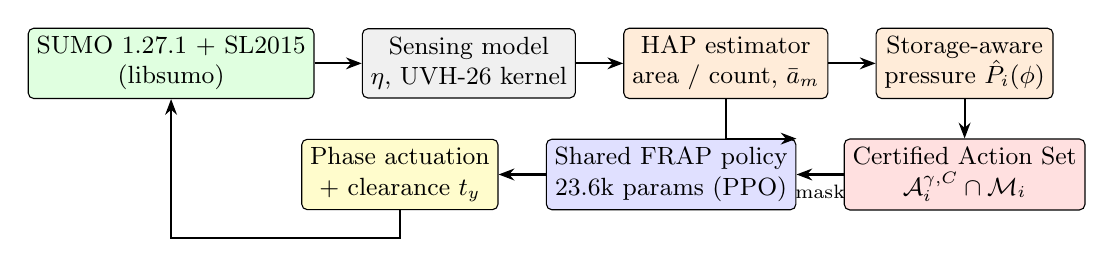
\begin{tikzpicture}[node distance=5mm and 6mm, font=\small,
  b/.style={draw,rounded corners=2pt,align=center,minimum height=8mm,inner sep=3pt},
  a/.style={-{Stealth[length=2mm]},thick}]
\node[b,fill=green!12] (sumo) {SUMO 1.27.1 + SL2015\\(libsumo)};
\node[b,fill=gray!12,right=of sumo] (sense) {Sensing model\\$\eta$, UVH-26 kernel};
\node[b,fill=orange!15,right=of sense] (est) {HAP estimator\\area / count, $\bar a_m$};
\node[b,fill=orange!15,right=of est] (press) {Storage-aware\\pressure $\hat P_i(\phi)$};
\node[b,fill=red!12,below=of press] (cas) {Certified Action Set\\$\mathcal A_i^{\gamma,C}\cap\mathcal M_i$};
\node[b,fill=blue!12,left=of cas] (pol) {Shared FRAP policy\\23.6k params (PPO)};
\node[b,fill=yellow!20,left=of pol] (act) {Phase actuation\\+ clearance $t_y$};
\draw[a] (sumo)--(sense); \draw[a] (sense)--(est); \draw[a] (est)--(press);
\draw[a] (press)--(cas); \draw[a] (est.south) |- (pol.north east);
\draw[a] (cas)--node[below,font=\scriptsize]{mask}(pol); \draw[a] (pol)--(act);
\draw[a] (act.south) -- ++(0,-0.35) -| (sumo.south);
\end{tikzpicture}}
\end{center}

% =============================================================================
\section{Real-data grounding with UVH-26 (GPU track)}
\label{sec:vision}
% =============================================================================
\begin{enumerate}
\item \textbf{Composition (cited fleet mix).} Map 14 classes to 5 model classes:
      2W$\leftarrow$two-wheeler (+bicycle reported separately);
      auto$\leftarrow$three-wheeler;
      car$\leftarrow$hatchback, sedan, SUV, MUV, van;
      bus$\leftarrow$bus, mini-bus, tempo-traveller;
      truck$\leftarrow$truck, LCV.
      Report shares by count and by box area, with bootstrap CIs over images. These are
      \emph{in-view} (occupancy) shares, which is exactly the queue-composition notion the
      estimator needs (P1c-9). Flow shares differ; state this.
\item \textbf{Detector noise.} Run the released UVH-26 detectors on the validation split
      (on the GPU). Match predictions to ground truth (IoU $\ge0.5$) to obtain the
      $5\times5$ confusion matrix, per-class recall (dropout $q_v$) and a count-error
      distribution vs crowd density. Fit $(\theta,q)$ and the empirical kernel $U_{\rm emp}$.
\item \textbf{Lemma 1 on real frames.} For each image, compare
      $\sum_{\rm boxes}\tilde a/\bar a$ with $\sum_v\rho_v n_v$, where $\tilde a$ is the box
      area normalised by the image's median car-box area, a perspective proxy. Report the
      dispersion of this ratio under HCM and area weights. This is an \emph{upper bound} on
      the field $\varepsilon$, because perspective variation inflates it. Per-camera
      calibration would remove the uniform part, which is free by Remark~3.
\item \textbf{Deliverables:} \file{vision/uvh26_*.py} scripts (no notebooks in the
      pipeline), numbers written to the config, and a data card with licence and citation.
\end{enumerate}
\textbf{Limits to state:} 2D image boxes are not ground-plane area; no camera IDs; daytime
frames only (06:00--18:00); February 2025 only.

% =============================================================================
\section{Scenarios}
\label{sec:scen}
% =============================================================================
\begin{description}[leftmargin=0pt]
\item[S1 Arterial (keep).] 5 signals, 400\,m. Recalibrate capacity after the fix.
\item[S2 Grid (keep).] $4\times4$, 300\,m. This is the spillback-prone case where HAP shows
  directional AQL and spillback gains (P1c-4).
\item[S3 Bengaluru OSM-informed corridor (rebuild).] Use the 5 verified Old Madras Road
  signals (\texttt{416419153}, \texttt{cluster\_11165270540\_\dots}, \texttt{442438288},
  \texttt{343459489}, \texttt{1837297484}; span 5.7\,km). Take real coordinates, spacing,
  approach lane counts and turn pockets from OSM and satellite imagery, but build the
  network \emph{programmatically} (plain \file{nod/edg/con} XML) so that the 62\% short
  single-lane segment problem never arises. Use a directional AM peak and the UVH-26
  composition. Document it as ``real geometry, abstracted topology'', a common and accepted
  practice.
\item[S4 Generalisation (optional, if time).] A RESCO real-world SUMO network (Ingolstadt7
  or Cologne8) with the Indian fleet injected, for zero-shot transfer.
\item[Stress variants.] v/c $\in\{0.85,0.95,1.05\}$, a 15-min surge, a lane-closure
  incident, 2W share $\pm10$\,pp, composition dispersion $\{0,.25,.5,.75,1\}$, and a
  bus-heavy approach.
\end{description}

% =============================================================================
\section{Baselines and fidelity gate}
\label{sec:baselines}
% =============================================================================
\small
\begin{tabularx}{\textwidth}{@{}lXl@{}}
\toprule
Group & Methods & Status \\
\midrule
Classical & Fixed-time (Webster on true demand), SOTL / SUMO actuated, MP (count),
  Efficient-MP, Advanced-MP (corrected), GreedyHAP, storage-aware GreedyHAP & exist \\
Finite-storage MP & \textbf{CABP} (Gregoire et al.\ 2015), \textbf{PWBP} (Li \& Jabari
  2019) or Hao et al.\ (2020) & new \\
Learned & IPPO, MPLight, PressLight, CoLight (\emph{full} multi-head GAT, not single-hop),
  Advanced-MPLight (running demand as current-phase stay bonus, as published) & code exists,
  fix + retrain \\
Stability-preserving RL & \textbf{Com-MP} adapted (shared MAPPO mixes count-MP and HAP
  pressures), code at \texttt{github.com/bryan-zjc/Com-MP} & new \\
Optional SOTA & Unicorn (2025, code public) if the fidelity gate can be met within 1 week & optional \\
Ours (ablations) & HAPLight-RL with CAS / with v2 filter / unconstrained; $(\gamma,C)$
  sweep; storage-aware off; no neighbour info; no domain randomisation; per-intersection
  networks & new \\
\bottomrule
\end{tabularx}
\normalsize

\paragraph{Fidelity gate (must pass before any baseline enters a table).}
\begin{enumerate}
\item Each learned baseline is trained on a \emph{homogeneous-traffic standard benchmark}
      (RESCO \texttt{grid4x4} / \texttt{arterial4x4} in SUMO). Its learning curve and its
      ranking relative to MP and fixed-time must be consistent with published results.
      If not, the port is fixed or the method is dropped, with the reason recorded.
\item A \textbf{reward gate v2} is pre-registered \emph{before} any v3 run. A reward passes
      if its episode return rank-correlates with $-$AQL (vehicle units) at
      $\rho\ge0.9$, over $\ge7$ controllers and $\ge3$ seeds. Throughput is excluded when its
      spread is under 1\% (the degenerate S2 criterion, P5-4). Each baseline trains with its
      \emph{published} reward if that passes; otherwise with \texttt{total\_queue}. This is
      declared a priori.
\item \textbf{Equal tuning budget.} Every learned method, ours included, gets the same small
      grid (learning rate $\{1,3\}\times10^{-4}$ $\times$ entropy $\{0.01,0.003\}$) on S1,
      selected on validation seeds that are disjoint from test seeds. All methods share the
      same iteration budget, fixed as $\max(40,\,2.5\times\text{post-fix knee})$.
\end{enumerate}

% =============================================================================
\section{Pre-registered hypotheses and experiment matrix}
\label{sec:stats}
% =============================================================================
\textbf{Minimum practically relevant effect (MPE):} 2\% ATT, 5\% AQL (unchanged from v2).
Each experiment gets \file{experiments/EXX/prereg.md}, committed and git-tagged before
launch. Refutations are reported.

\small
\begin{longtable}{@{}p{0.9cm}p{6.7cm}p{8.2cm}@{}}
\toprule
ID & Hypothesis & Test / decision rule \\
\midrule
\endhead
H1 & HAP$-$MP advantage (AQL in vehicle and weighted units, spillback time) grows with
     composition dispersion and is zero at zero dispersion. &
     Paired $n=20$ per level, 5 levels, S2 and S3. Page / Spearman trend test. A null result
     is reported as a boundary of the contribution. \\
H2 & HAPLight-RL (CAS) beats greedy HAP by $\ge$MPE on ATT in every scenario, and beats
     every learned baseline. &
     Wilcoxon + Holm per (scenario, metric) family, rank-biserial, hierarchical BCa. \\
H3 & HAPLight-RL degrades more slowly with $\eta$ than count-based methods, including
     $\eta\in\{0.8,1.0\}$ (out of distribution) and the UVH-26 real-calibrated condition. &
     Slope of relative ATT vs $\eta$; bootstrap CI on the slope difference. \\
H4 & CAS costs $\le$MPE at nominal demand and lowers deadlock under stress. &
     TOST non-inferiority vs unconstrained RL (margin = MPE); McNemar on paired deadlock
     events. \\
H5 & Weight-vector trade-off: area is better for the estimator, HCM for A5. &
     C1/C2 with $\ge$5 seeds plus UVH-26; $\varepsilon+\nu$ with CIs; control performance in
     a $2\times2$ (weights $\times$ estimator). \\
H6 & Storage-aware pressure cuts the deadlock rate vs MP and HAP at $\le$MPE nominal cost. &
     $n=200$ paired stress episodes per cell (powered for 5\% vs 1\%), McNemar, Wilson CIs. \\
H7 & A policy trained on S1+S2 transfers zero-shot to S3 (and S4) and retains its sign of
     advantage over greedy HAP. &
     Paired $n=20$; report the retained fraction of the in-domain gain. \\
\bottomrule
\end{longtable}
\normalsize

\small
\begin{longtable}{@{}p{0.7cm}p{5.0cm}p{5.6cm}p{4.4cm}@{}}
\toprule
Exp. & Content & Design & Output \\
\midrule
\endhead
E0 & Re-validation after the 8$\times$ fix & C1/C2 (5 seeds), capacity scales,
  $\bar a_m$ refit, $B$, storage threshold & corrected config + decision record \\
E1 & Main comparison & S1--S3 $\times$ $\eta\in\{0,0.6\}$ $\times$ all methods; 3--5 training
  seeds $\times$ 20 evaluation seeds & Table (main), effect sizes \\
E2 & H1 dose--response & 5 dispersion levels, paired, S2/S3 & Figure + trend test \\
E3 & Robustness & $\eta\in\{0,.2,.4,.6,.8,1\}$ + UVH-26 kernel, S2/S3 & Robustness curves \\
E4 & Deadlock power study & v/c 0.95/1.05 + surge, 200 paired episodes per cell, 6 methods & Deadlock table \\
E5 & Ablations & CAS / filter / none; $(\gamma,C)$ grid; storage-aware off; neighbours off;
  domain randomisation off; IPPO; reward forms; $c_{\rm sw}=0$ & Ablation table, $(\gamma,C)$ frontier \\
E6 & Weight vector (H5) & HCM vs area $\times$ count vs area estimator & $2\times2$ table \\
E7 & Fairness & per-class AWT, Gini, PWD; 2W penalty check & Fairness table \\
E8 & Sensitivity & $\Delta t\in\{5,10\}$, $B$ or $C$, $\pm20\%$ equivalency, 2W $\pm10$\,pp,
  bus occupancy & Sensitivity figure \\
E9 & Generalisation & zero-shot S3/S4, unseen demand profiles & Transfer table \\
E10 & Deployability & ONNX CPU latency, parameter count, sensing bytes per $\Delta t$ & Text + table \\
T  & Theorem checks & store-and-forward simulator: CAS bounded inside
  $(1-\gamma)\Lambda$, divergent outside; measured vs predicted bound & Appendix figure, CI test \\
\bottomrule
\end{longtable}
\normalsize

\paragraph{Statistics.}
\begin{itemize}
\item \textbf{Nested design.} Training seed $\supset$ evaluation seed, so CIs use a
      \emph{hierarchical bootstrap}: resample training seeds, then evaluation seeds.
\item \textbf{Location and tests.} Medians are primary (heavy tails from deadlock episodes).
      Wilcoxon with Holm correction within each (scenario, metric) family; rank-biserial
      $r$; BCa 95\% CIs.
\item \textbf{Rare events.} Wilson CIs for rates and McNemar for paired deadlock.
\item \textbf{Non-inferiority.} TOST.
\item \textbf{Reporting.} \file{eval/stats.py} and \file{eval/report.py} emit every LaTeX
      table. No number is ever typed by hand.
\end{itemize}

% =============================================================================
\section{Compute plan}
% =============================================================================
\textbf{Measured today (TraCI, system Python, OneDrive):} one PPO iteration (8 parallel
3600\,s episodes plus update) takes $\approx$430\,s on S1 and $\approx$750\,s on S2.
Evaluation episodes take $\approx$220--250\,s (S1) and $\approx$340\,s (S2) each.

\textbf{Expected after Phase A:} libsumo, off OneDrive, one environment. The 1.5--2.5$\times$
speed-up must be \emph{measured} before the budget below is locked.

\small
\begin{tabularx}{\textwidth}{@{}Xrr@{}}
\toprule
Block (40 iterations, 3 training seeds) & current (h) & after Phase A, est.\ 2$\times$ (h) \\
\midrule
Main learned set: 8 methods $\times$ S1+S2 $\times$ 3 seeds (S1 $\approx$5\,h, S2 $\approx$8.5\,h per run) & 324 & 162 \\
Ablations on S2: 6 variants $\times$ 3 seeds & 153 & 77 \\
S3 training: 4 methods $\times$ 3 seeds & 72 & 36 \\
Evaluation: all experiments, $\approx$7{,}500 episodes at 6 workers & 85 & 43 \\
Theory simulator, UVH-26 inference (GPU), re-validation & 15 & 15 \\
\midrule
\textbf{Total} & \textbf{649} ($\approx$27 days) & \textbf{333} ($\approx$14 days) \\
\bottomrule
\end{tabularx}
\normalsize

\paragraph{Compute tiers.}
\begin{description}
\item[Tier 1, laptop only, after Phase A.] $\approx$14 days of continuous compute. This
  fits the 12-week plan only if the queue never idles.
\item[Tier 2, plus RAM upgrade to 16--32 GB.] 12--14 workers instead of 6--8, an extra
  $\approx$1.5$\times$, giving $\approx$9--10 days. \textbf{Recommended.}
\item[Tier 3, cloud or HPC burst for E1 and E5.] A 32--64 vCPU instance, or the RGIPT
  cluster, running 4--6 runs concurrently. The sweep finishes in 3--4 days. Price it at the
  time of booking.
\end{description}

\textbf{Cut order if over budget:} (1) S4 and Unicorn; (2) ablations down to 2 seeds;
(3) robustness grid on S2 only; (4) evaluation seeds 20$\to$15. Never: training seeds below 3,
or unequal budgets.

% =============================================================================
\section{Repository blueprint and engineering practices}
\label{sec:repo}
% =============================================================================
\subsection{Location and layout}
Code in \texttt{C:\textbackslash dev\textbackslash haplight} (NVMe, not synced). Bulk
artefacts in \texttt{D:\textbackslash haplight-data} via the environment variable
\texttt{HAPLIGHT\_DATA}. A private GitHub remote. OneDrive only receives weekly zipped
snapshots. The current folder is frozen as
\texttt{D:\textbackslash haplight-archive\textbackslash HAPLIGHT\_v2\_2026-11-04.zip} and
its changelog is imported as \file{docs/history/}.

{\footnotesize
\begin{verbatim}
haplight/
  pyproject.toml  uv.lock  README.md  CLAUDE.md  CITATION.cff  LICENSE
  .pre-commit-config.yaml  .github/workflows/ci.yml  .gitignore
  configs/           base.yaml + scenario/*.yaml + experiment/*.yaml  (pydantic-validated)
  src/haplight/
    sim/             env.py, measurement.py, topology.py, backend.py (libsumo|traci)
    hap/             weights.py, estimators.py, pressure.py, storage.py
    sensing/         noise.py, kernels.py (synthetic + UVH-26 empirical)
    control/         classical.py (FT,SOTL,MP,EMP,AMP,CABP,PWBP,GreedyHAP), cas.py, filter.py
    rl/              policy.py, ppo.py, rollout.py, train.py
    baselines/       mplight.py, presslight.py, colight.py, amplight.py, ippo.py, commp.py
    theory/          sfsim.py  (fast store-and-forward simulator for theorem checks)
    eval/            runner.py, metrics.py, stats.py, report.py
    vision/          uvh26_composition.py, uvh26_confusion.py, uvh26_area.py
    utils/           seeding.py, manifest.py, io.py, log.py
  scripts/           thin CLIs only (train, evaluate, calibrate, build_nets, report)
  experiments/E00..E10/   prereg.md, config.yaml, analysis.py
  nets/              s1, s2, s3_bengaluru (generated, with build provenance)
  tests/unit  tests/integration  tests/regression
  paper/             LaTeX; paper/generated/ (tables from report.py only)
  docs/              plan/, decisions/ (ADR), STATUS.md, history/
\end{verbatim}
}

\subsection{Practices (each fixes a failure observed in v2)}
\small
\begin{longtable}{@{}p{6.4cm}p{9.6cm}@{}}
\toprule
Practice & Why (observed failure) \\
\midrule
\endhead
One \texttt{uv}-locked environment, Python 3.12, SUMO 1.27.1 everywhere & Two divergent
  environments; training silently ran traci 1.25 against the 1.27.1 binary. \\
libsumo backend + \texttt{test\_backend\_parity} (traci vs libsumo, same seed $\Rightarrow$
  identical trajectory) & Socket crash (13 Sep); 2--3$\times$ speed. \\
Fresh process per episode (\texttt{maxtasksperchild=1}) enforced by a structural test &
  State leakage across episodes, confirmed six times (P4c-14/15). \\
Ground-truth measurement gate in CI (\texttt{test\_counts\_match\_ground\_truth}) &
  The 8$\times$ double-counting bug survived because tests compared counts with counts. \\
Every run writes \file{manifest.json}: git SHA, dirty flag, config hash, seed, package
  versions, backend, measurement-pipeline version, host, wall-clock & Pre- and post-fix
  runs were compared by mistake (P5-3 retraction). Comparisons across pipeline versions are
  refused by code. \\
Results as parquet, one row per episode, plus a run index & Results scattered across
  JSON, CSV and stdout files. \\
Pre-registration file + git tag before each experiment & Threshold and gate decisions were
  made after seeing data and had to be retracted. \\
\file{docs/STATUS.md} updated at the end of every session; ADR decision records & This
  session started with no knowledge of where work stopped. \\
\file{CLAUDE.md} with the project rules (no paper edits during experiments, config is the
  single source of numbers, gates, cooldowns, never touch the user's processes) & Keeps AI
  development sessions consistent. \\
ruff (lint + format), mypy (gradual), pytest markers (\texttt{unit}, \texttt{sumo},
  \texttt{slow}), pre-commit, GitHub Actions (unit + lint on every push; SUMO integration
  nightly) & Prevent regressions; the suite takes 16 min, so split it by marker. \\
Long runs: chain scripts with retry watchdog, cooldowns, resumable checkpoints, logs on D:
  & Laptop throttling, socket failures, OneDrive contention. \\
\bottomrule
\end{longtable}
\normalsize

\subsection{Migration from the v2 folder}
\begin{enumerate}
\item Archive the folder (zip, read-only) and record SHA-256 checksums of the valid
      checkpoints.
\item Port modules into the package layout \emph{without behaviour change}. The ported
      tests (84) must pass bit-identically on the same backend first, then on libsumo.
\item Port configs, nets and the valid evidence (P5-5 numbers) as regression fixtures.
\item Only then start v3 feature work (CAS, storage theory, vision, baselines).
\end{enumerate}

% =============================================================================
\section{Timeline and gates}
% =============================================================================
\small
\begin{longtable}{@{}p{1.6cm}p{2.9cm}p{7.2cm}p{4.0cm}@{}}
\toprule
Weeks & Dates (2026--27) & Work & Gate to pass \\
\midrule
\endhead
1 & 9--15 Nov & Repo + env + CI; backend parity; speed benchmark; port v2 code;
  download UVH-26 to D:; RAM upgrade ordered & 84 tests green on libsumo; parity holds;
  speed-up measured \\
2 & 16--22 Nov & E0 re-validation; UVH-26 composition + confusion; CAS implementation +
  unit tests; theory drafts P1--P4; S3 rebuild started & E0 decision record; CAS tests;
  composition table \\
3 & 23--29 Nov & Store-and-forward theorem checks; HAPLight-RL-CAS pilot (S1, 3 seeds);
  CABP/PWBP; reward gate v2 & Pilot beats greedy HAP; theorem check passes \\
4--5 & 30 Nov--13 Dec & Baseline fidelity gates on RESCO; Com-MP adaptation; equal HP tuning;
  S3 calibration; finite-storage theorem time box & All baselines gated; S3 loads, MP beats
  FT under stress \\
6--8 & 14 Dec--3 Jan & E1 + E5 training sweep (Tier 2 or 3 compute) & All checkpoints
  present with manifests \\
9 & 4--10 Jan & E2--E4, E6--E10 evaluations & All parquet present \\
10 & 11--17 Jan & \file{stats.py}/\file{report.py}; results review; narrative decision
  (author review) & Every table generated \\
11--12 & 18--31 Jan & Paper v3 rewrite (from the decision log + generated tables);
  internal review; arXiv & 0 placeholders; every proof independently re-checked \\
13 & early Feb 2027 & Submit (IEEE T-ITS or TR-C) & --- \\
\bottomrule
\end{longtable}
\normalsize

% =============================================================================
\section{Risk register}
% =============================================================================
\small
\begin{tabularx}{\textwidth}{@{}p{4.6cm}cX@{}}
\toprule
Risk & Likelihood & Mitigation \\
\midrule
H1 null: HAP $\approx$ MP on delay & high & Already likely. Reframe HAP as the correct
  units for stability (A5) and sensing (Lemma~1). Gains are claimed from CAS-RL and
  storage-awareness. Report H1 as a boundary result. \\
Finite-storage theorem not provable in time & med--high & 3-week time box, then fall back
  to proposition + powered study. The gap is open in the 2026 literature. \\
Overlap with Com-MP or another preprint appears & medium & Cite, compare as a baseline,
  stress the differentiators (vehicle heterogeneity, sensing theory, real data). Post to
  arXiv as soon as E1 is done. \\
Compute overrun & medium & Tiers 2/3; cut order; shared iteration budget. \\
Baseline-port criticism & medium & Fidelity gate on RESCO; published-reward variants; equal
  tuning budget. \\
CAS too restrictive (RL $\approx$ greedy) & medium & The $(\gamma,C)$ frontier is itself a
  result. Choose the operating point on validation seeds only. \\
Backend non-determinism / crashes & low--med & Parity test; retry watchdog; fresh process
  per episode. \\
Another measurement bug & low & Ground-truth gate in CI; pipeline version in manifests. \\
Loss of session context & medium & \file{STATUS.md}, ADRs and \file{CLAUDE.md}; commit and
  push every session. \\
UVH-26 analysis challenged (2D boxes, no camera IDs) & medium & Present as an
  upper-bound/approximate validation with the limits stated. \\
\bottomrule
\end{tabularx}
\normalsize

% =============================================================================
\section{Immediate next steps (first two weeks)}
\label{sec:next}
% =============================================================================
\begin{keybox}[Decisions taken on 4 November 2026]
\begin{enumerate}[leftmargin=*]
\item \textbf{Repository:} code in \texttt{C:\textbackslash dev\textbackslash haplight}
      (\url{https://github.com/jarvisxys/haplight}), data in
      \texttt{D:\textbackslash haplight-data}. The v2 folder is archived in
      \texttt{D:\textbackslash haplight-data\textbackslash archive}.
\item \textbf{No RAM upgrade.} The laptop is for development, tests and small pilots (Tier~1).
\item \textbf{Heavy compute} (E1, E4, E5) runs on the college server with an NVIDIA RTX PRO
      6000 Blackwell (96\,GB); this replaces the cloud burst of Tier~3. SUMO is CPU-bound, so
      throughput depends on the server's CPU core count and RAM (to be confirmed). The GPU
      serves the UVH-26 vision track and needs a PyTorch build with CUDA~12.8 or later.
\item \textbf{Main contribution:} the Certified Action Set replaces the safety filter, which
      stays as an ablation.
\item \textbf{Authorship:} single author for now (Aditya Kumar); co-authors to be added later.
\end{enumerate}
\end{keybox}
\begin{enumerate}
\item \textbf{Decide}: repository location (proposed \texttt{C:\textbackslash dev}
      + \texttt{D:\textbackslash haplight-data}), the GitHub remote, the RAM upgrade, and
      whether a cloud or HPC burst is available.
\item Snapshot the current folder (git-init plus zip archive). Do \emph{not} resume
      \file{_phase5_retrain4.sh}; v3 supersedes it.
\item Create the v3 repository and \texttt{uv} environment. Port the code and tests. Run
      the parity test and the speed benchmark.
\item Run E0 re-validation (C1/C2 seeded, capacity, $\bar a_m$, filter $B$).
\item Download UVH-26 (validation split + all annotation JSON) to D:. Compute the
      composition and the detector confusion matrix on the GPU.
\item Implement \file{control/cas.py} and its tests (argmax $\in$ CAS; CAS(0,0) $\equiv$
      greedy; mask never empty) and \file{theory/sfsim.py}.
\item Draft Theorem~2 (CAS) and Proposition~3 (storage) with proof
      obligations P1--P4.
\item Pilot HAPLight-RL-CAS on S1 (3 seeds, 40 iterations) against greedy HAP.
\item Write and tag \file{experiments/E01/prereg.md} and reward gate v2.
\item Start the S3 OSM-informed corridor build.
\end{enumerate}

% =============================================================================
\appendix
\section{Key references (verified during this audit)}
% =============================================================================
\small
\begin{enumerate}[label={[\arabic*]},leftmargin=*]
\item J.~Zhu, C.~Tan, ``Stability-preserving reinforcement learning for heterogeneity-aware
  composite max-pressure traffic signal control (Com-MP),'' arXiv:2610.31037, Oct 2026.
  \url{https://arxiv.org/abs/2610.31037}
\item C.~Tan, ``Decision timescales in max-pressure traffic signal control: theory,
  methodology, and validation (VT-MP),'' arXiv:2610.32280, Oct 2026.
  \url{https://arxiv.org/abs/2610.32280}
\item ``PASCAL: Pressure Adaptive Signal Control ALgorithm,'' Transp.\ Res.\ Part C, 2026.
  \url{https://www.sciencedirect.com/science/article/pii/S0968090X26002925}
\item C.~Tan et al., ``CV-MP: max-pressure control in heterogeneously distributed and
  partially connected vehicle environments,'' Transp.\ Res.\ Part B 204:103387, 2026;
  arXiv:2505.05258.
\item C.~Tan et al., ``Transit-MP,'' arXiv:2511.00309, 2025.
\item T.~Ahmed, H.~Liu, V.~Gayah, ``OCC-MP: a max-pressure framework to prioritize transit
  and high occupancy vehicles,'' Transp.\ Res.\ Part C 166:104795, 2024.
\item H.~Liu, V.~Gayah, M.~Levin, ``A max pressure algorithm for traffic signals considering
  pedestrian queues,'' Transp.\ Res.\ Part C 169:104865, 2024; arXiv:2406.19305.
\item J.~Gregoire, X.~Qian, E.~Frazzoli, A.~de~La~Fortelle, T.~Wongpiromsarn,
  ``Capacity-aware backpressure traffic signal control,'' IEEE TCNS 2(2):164--173, 2015;
  arXiv:1309.6484.
\item L.~Li, S.~Jabari, ``Position weighted backpressure intersection control for urban
  networks,'' Transp.\ Res.\ Part B 128:435--461, 2019; arXiv:1810.11406.
\item N.~Xiao et al., ``Pressure releasing policy in traffic signal control with finite
  queue capacities,'' IEEE CDC, 2014.
\item T.~Charalambous et al., ``Back-pressure traffic signal control in the presence of
  noisy queue information,'' IFAC-PapersOnLine 56, 2023.
\item P.~Varaiya, ``Max pressure control of a network of signalized intersections,''
  Transp.\ Res.\ Part C 36:177--195, 2013.
\item T.~Le et al., ``Decentralized signal control for urban road networks,'' Transp.\ Res.\
  Part C 58:431--450, 2015.
\item M.~J.~Neely, \emph{Stochastic Network Optimization with Application to Communication
  and Queueing Systems}, Morgan \& Claypool, 2010.
\item X.~Wang et al., ``Learning the max pressure control for urban traffic networks
  considering the phase switching loss,'' Transp.\ Res.\ Part C 140:103670, 2022.
\item L.~Zhang et al., ``Expression might be enough: representing pressure and demand for
  RL-based traffic signal control (Advanced-XLight),'' ICML 2022; arXiv:2112.10107.
\item ``Unicorn: a universal and collaborative RL approach towards generalizable
  network-wide traffic signal control,'' arXiv:2503.11488, 2025.
\item S.~Lai et al., ``LLMLight: large language models as traffic signal control agents,''
  arXiv:2312.16044.
\item J.~Ault, G.~Sharon, ``Reinforcement learning benchmarks for traffic signal control
  (RESCO),'' NeurIPS Datasets \& Benchmarks, 2021.
\item H.~Mei et al., ``LibSignal: an open library for traffic signal control,'' Machine
  Learning 113:5235--5271, 2024; arXiv:2211.10649.
\item ``Sim2Signal: sim-to-real benchmarks for traffic signal control,'' arXiv:2609.01676,
  2026.
\item A.~Agarwal et al., ``Dynamic traffic signal control for heterogeneous traffic
  conditions using max pressure and reinforcement learning,'' Expert Syst.\ Appl., 2024.
  \url{https://www.sciencedirect.com/science/article/abs/pii/S095741742401282X}
\item A.~Sharma et al., ``The Urban Vision Hackathon dataset and models: towards image
  annotations and accurate vision models for Indian traffic (UVH-26),'' arXiv:2511.02563,
  2025. Data: \url{https://huggingface.co/datasets/iisc-aim/UVH-26}
\item ``A gain-modulated max pressure control for port collection and distribution road
  networks (PCU-weighted MP),'' Systems 14(3):332, 2026.
\item Area-occupancy PCU for Indian mixed traffic, J.\ Transp.\ Eng., 2018.
  \url{https://ascelibrary.com/doi/10.1061/JTEPBS.0000184}
\end{enumerate}
\normalsize

\section{Glossary of project-specific terms}
\small
\begin{description}[leftmargin=0pt,itemsep=1pt]
\item[8$\times$ bug (P5-2)] Context subscriptions counted every vehicle once per
  overlapping edge context. Fixed by deduplicating by vehicle ID; guarded by a ground-truth
  test.
\item[S1 / S2 / S3] 5-signal arterial / $4\times4$ grid / Bengaluru corridor.
\item[$\eta$] Composite sensing-noise level in $[0,1]$. Training draws
  $\eta\sim\mathcal U[0,0.6]$.
\item[\texttt{total\_queue}] Reward $-\frac{1}{x_{\rm ref}}\sum_{m\in\mathcal M_i}x_m$
  (true channel), validated by the reward gate.
\item[Gridlock / deadlock] Binary per episode: SUMO still has pending (un-inserted)
  vehicles at truncation, \texttt{env.pending\_count()}$\,>0$ (the evaluator's
  \texttt{GRIDLOCK\_KEY}). The diagnostic signature is worst-movement storage occupancy pinned
  above 100\%. v3 should pre-register this definition, plus a continuous severity measure.
\end{description}

\end{document}
